\documentclass[1p]{elsarticle_modified}
%\bibliographystyle{elsarticle-num}

%\usepackage[colorlinks]{hyperref}
%\usepackage{abbrmath_seonhwa} %\Abb, \Ascr, \Acal ,\Abf, \Afrak
\usepackage{amsfonts}
\usepackage{amssymb}
\usepackage{amsmath}
\usepackage{amsthm}
\usepackage{scalefnt}
\usepackage{amsbsy}
\usepackage{kotex}
\usepackage{caption}
\usepackage{subfig}
\usepackage{color}
\usepackage{graphicx}
\usepackage{xcolor} %% white, black, red, green, blue, cyan, magenta, yellow
\usepackage{float}
\usepackage{setspace}
\usepackage{hyperref}

\usepackage{tikz}
\usetikzlibrary{arrows}

\usepackage{multirow}
\usepackage{array} % fixed length table
\usepackage{hhline}

%%%%%%%%%%%%%%%%%%%%%
\makeatletter
\renewcommand*\env@matrix[1][\arraystretch]{%
	\edef\arraystretch{#1}%
	\hskip -\arraycolsep
	\let\@ifnextchar\new@ifnextchar
	\array{*\c@MaxMatrixCols c}}
\makeatother %https://tex.stackexchange.com/questions/14071/how-can-i-increase-the-line-spacing-in-a-matrix
%%%%%%%%%%%%%%%

\usepackage[normalem]{ulem}

\newcommand{\msout}[1]{\ifmmode\text{\sout{\ensuremath{#1}}}\else\sout{#1}\fi}
%SOURCE: \msout is \stkout macro in https://tex.stackexchange.com/questions/20609/strikeout-in-math-mode

\newcommand{\cancel}[1]{
	\ifmmode
	{\color{red}\msout{#1}}
	\else
	{\color{red}\sout{#1}}
	\fi
}

\newcommand{\add}[1]{
	{\color{blue}\uwave{#1}}
}

\newcommand{\replace}[2]{
	\ifmmode
	{\color{red}\msout{#1}}{\color{blue}\uwave{#2}}
	\else
	{\color{red}\sout{#1}}{\color{blue}\uwave{#2}}
	\fi
}

\newcommand{\Sol}{\mathcal{S}} %segment
\newcommand{\D}{D} %diagram
\newcommand{\A}{\mathcal{A}} %arc


%%%%%%%%%%%%%%%%%%%%%%%%%%%%%5 test

\def\sl{\operatorname{\textup{SL}}(2,\Cbb)}
\def\psl{\operatorname{\textup{PSL}}(2,\Cbb)}
\def\quan{\mkern 1mu \triangleright \mkern 1mu}

\theoremstyle{definition}
\newtheorem{thm}{Theorem}[section]
\newtheorem{prop}[thm]{Proposition}
\newtheorem{lem}[thm]{Lemma}
\newtheorem{ques}[thm]{Question}
\newtheorem{cor}[thm]{Corollary}
\newtheorem{defn}[thm]{Definition}
\newtheorem{exam}[thm]{Example}
\newtheorem{rmk}[thm]{Remark}
\newtheorem{alg}[thm]{Algorithm}

\newcommand{\I}{\sqrt{-1}}
\begin{document}

%\begin{frontmatter}
%
%\title{Boundary parabolic representations of knots up to 8 crossings}
%
%%% Group authors per affiliation:
%\author{Yunhi Cho} 
%\address{Department of Mathematics, University of Seoul, Seoul, Korea}
%\ead{yhcho@uos.ac.kr}
%
%
%\author{Seonhwa Kim} %\fnref{s_kim}}
%\address{Center for Geometry and Physics, Institute for Basic Science, Pohang, 37673, Korea}
%\ead{ryeona17@ibs.re.kr}
%
%\author{Hyuk Kim}
%\address{Department of Mathematical Sciences, Seoul National University, Seoul 08826, Korea}
%\ead{hyukkim@snu.ac.kr}
%
%\author{Seokbeom Yoon}
%\address{Department of Mathematical Sciences, Seoul National University, Seoul, 08826,  Korea}
%\ead{sbyoon15@snu.ac.kr}
%
%\begin{abstract}
%We find all boundary parabolic representation of knots up to 8 crossings.
%
%\end{abstract}
%\begin{keyword}
%    \MSC[2010] 57M25 
%\end{keyword}
%
%\end{frontmatter}

%\linenumbers
%\tableofcontents
%
\newcommand\colored[1]{\textcolor{white}{\rule[-0.35ex]{0.8em}{1.4ex}}\kern-0.8em\color{red} #1}%
%\newcommand\colored[1]{\textcolor{white}{ #1}\kern-2.17ex	\textcolor{white}{ #1}\kern-1.81ex	\textcolor{white}{ #1}\kern-2.15ex\color{red}#1	}

{\Large $\underline{12a_{0308}~(K12a_{0308})}$}

\setlength{\tabcolsep}{10pt}
\renewcommand{\arraystretch}{1.6}
\vspace{1cm}\begin{tabular}{m{100pt}>{\centering\arraybackslash}m{274pt}}
\multirow{5}{120pt}{
	\centering
	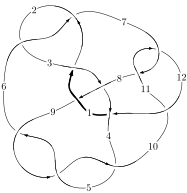
\includegraphics[width=112pt]{../../../GIT/diagram.site/Diagrams/png/1109_12a_0308.png}\\
\ \ \ A knot diagram\footnotemark}&
\allowdisplaybreaks
\textbf{Linearized knot diagam} \\
\cline{2-2}
 &
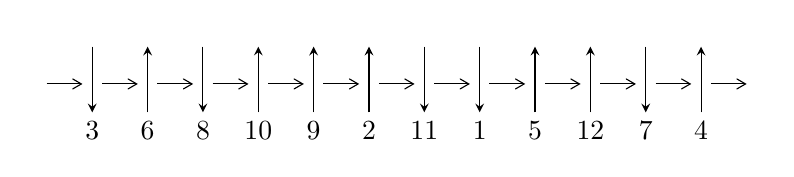
\begin{tikzpicture}[x=20pt, y=17pt]
	% nodes
	\node (C0) at (0, 0) {};
	\node (C1) at (1, 0) {};
	\node (C1U) at (1, +1) {};
	\node (C1D) at (1, -1) {3};

	\node (C2) at (2, 0) {};
	\node (C2U) at (2, +1) {};
	\node (C2D) at (2, -1) {6};

	\node (C3) at (3, 0) {};
	\node (C3U) at (3, +1) {};
	\node (C3D) at (3, -1) {8};

	\node (C4) at (4, 0) {};
	\node (C4U) at (4, +1) {};
	\node (C4D) at (4, -1) {10};

	\node (C5) at (5, 0) {};
	\node (C5U) at (5, +1) {};
	\node (C5D) at (5, -1) {9};

	\node (C6) at (6, 0) {};
	\node (C6U) at (6, +1) {};
	\node (C6D) at (6, -1) {2};

	\node (C7) at (7, 0) {};
	\node (C7U) at (7, +1) {};
	\node (C7D) at (7, -1) {11};

	\node (C8) at (8, 0) {};
	\node (C8U) at (8, +1) {};
	\node (C8D) at (8, -1) {1};

	\node (C9) at (9, 0) {};
	\node (C9U) at (9, +1) {};
	\node (C9D) at (9, -1) {5};

	\node (C10) at (10, 0) {};
	\node (C10U) at (10, +1) {};
	\node (C10D) at (10, -1) {12};

	\node (C11) at (11, 0) {};
	\node (C11U) at (11, +1) {};
	\node (C11D) at (11, -1) {7};

	\node (C12) at (12, 0) {};
	\node (C12U) at (12, +1) {};
	\node (C12D) at (12, -1) {4};
	\node (C13) at (13, 0) {};

	% arrows
	\draw[->,>={angle 60}]
	(C0) edge (C1) (C1) edge (C2) (C2) edge (C3) (C3) edge (C4) (C4) edge (C5) (C5) edge (C6) (C6) edge (C7) (C7) edge (C8) (C8) edge (C9) (C9) edge (C10) (C10) edge (C11) (C11) edge (C12) (C12) edge (C13) ;	\draw[->,>=stealth]
	(C1U) edge (C1D) (C2D) edge (C2U) (C3U) edge (C3D) (C4D) edge (C4U) (C5D) edge (C5U) (C6D) edge (C6U) (C7U) edge (C7D) (C8U) edge (C8D) (C9D) edge (C9U) (C10D) edge (C10U) (C11U) edge (C11D) (C12D) edge (C12U) ;
	\end{tikzpicture} \\
\hhline{~~} \\& 
\textbf{Solving Sequence} \\ \cline{2-2} 
 &
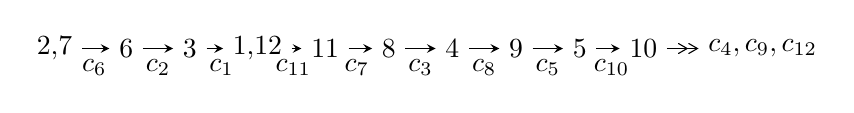
\begin{tikzpicture}[x=23pt, y=7pt]
	% node
	\node (A0) at (-1/8, 0) {2,7};
	\node (A1) at (1, 0) {6};
	\node (A2) at (2, 0) {3};
	\node (A3) at (49/16, 0) {1,12};
	\node (A4) at (33/8, 0) {11};
	\node (A5) at (41/8, 0) {8};
	\node (A6) at (49/8, 0) {4};
	\node (A7) at (57/8, 0) {9};
	\node (A8) at (65/8, 0) {5};
	\node (A9) at (73/8, 0) {10};
	\node (C1) at (1/2, -1) {$c_{6}$};
	\node (C2) at (3/2, -1) {$c_{2}$};
	\node (C3) at (5/2, -1) {$c_{1}$};
	\node (C4) at (29/8, -1) {$c_{11}$};
	\node (C5) at (37/8, -1) {$c_{7}$};
	\node (C6) at (45/8, -1) {$c_{3}$};
	\node (C7) at (53/8, -1) {$c_{8}$};
	\node (C8) at (61/8, -1) {$c_{5}$};
	\node (C9) at (69/8, -1) {$c_{10}$};
	\node (A10) at (11, 0) {$c_{4},c_{9},c_{12}$};

	% edge
	\draw[->,>=stealth]	
	(A0) edge (A1) (A1) edge (A2) (A2) edge (A3) (A3) edge (A4) (A4) edge (A5) (A5) edge (A6) (A6) edge (A7) (A7) edge (A8) (A8) edge (A9) ;
	\draw[->>,>={angle 60}]	
	(A9) edge (A10);
\end{tikzpicture} \\ 

\end{tabular} \\

\footnotetext{
The image of knot diagram is generated by the software ``\textbf{Draw programme}" developed by Andrew Bartholomew(\url{http://www.layer8.co.uk/maths/draw/index.htm\#Running-draw}), where we modified some parts for our purpose(\url{https://github.com/CATsTAILs/LinksPainter}).
}\phantom \\ \newline 
\centering \textbf{Ideals for irreducible components\footnotemark of $X_{\text{par}}$} 
 
\begin{align*}
I^u_{1}&=\langle 
-6.76624\times10^{219} u^{125}-7.53327\times10^{220} u^{124}+\cdots+1.14785\times10^{220} b-1.35671\times10^{222},\\
\phantom{I^u_{1}}&\phantom{= \langle  }5.17876\times10^{220} u^{125}+9.23238\times10^{220} u^{124}+\cdots+1.14785\times10^{220} a+4.07465\times10^{219},\\
\phantom{I^u_{1}}&\phantom{= \langle  }u^{126}+u^{125}+\cdots+34 u+14\rangle \\
I^u_{2}&=\langle 
6 u^{25}+6 u^{24}+\cdots+b-1,\;u^{25}+18 u^{24}+\cdots+2 a+13,\;u^{26}+2 u^{25}+\cdots- u+2\rangle \\
\\
\end{align*}
\raggedright * 2 irreducible components of $\dim_{\mathbb{C}}=0$, with total 152 representations.\\
\footnotetext{All coefficients of polynomials are rational numbers. But the coefficients are sometimes approximated in decimal forms when there is not enough margin.}
\newpage
\renewcommand{\arraystretch}{1}
\centering \section*{I. $I^u_{1}= \langle -6.77\times10^{219} u^{125}-7.53\times10^{220} u^{124}+\cdots+1.15\times10^{220} b-1.36\times10^{222},\;5.18\times10^{220} u^{125}+9.23\times10^{220} u^{124}+\cdots+1.15\times10^{220} a+4.07\times10^{219},\;u^{126}+u^{125}+\cdots+34 u+14 \rangle$}
\flushleft \textbf{(i) Arc colorings}\\
\begin{tabular}{m{7pt} m{180pt} m{7pt} m{180pt} }
\flushright $a_{2}=$&$\begin{pmatrix}0\\u\end{pmatrix}$ \\
\flushright $a_{7}=$&$\begin{pmatrix}1\\0\end{pmatrix}$ \\
\flushright $a_{6}=$&$\begin{pmatrix}1\\u^2\end{pmatrix}$ \\
\flushright $a_{3}=$&$\begin{pmatrix}u\\u^3+u\end{pmatrix}$ \\
\flushright $a_{1}=$&$\begin{pmatrix}u^3\\u^5+u^3+u\end{pmatrix}$ \\
\flushright $a_{12}=$&$\begin{pmatrix}-4.51170 u^{125}-8.04318 u^{124}+\cdots-101.412 u-0.354980\\0.589470 u^{125}+6.56293 u^{124}+\cdots+423.567 u+118.196\end{pmatrix}$ \\
\flushright $a_{11}=$&$\begin{pmatrix}-3.92223 u^{125}-1.48025 u^{124}+\cdots+322.156 u+117.841\\0.589470 u^{125}+6.56293 u^{124}+\cdots+423.567 u+118.196\end{pmatrix}$ \\
\flushright $a_{8}=$&$\begin{pmatrix}7.01915 u^{125}+19.5025 u^{124}+\cdots+898.354 u+202.158\\8.43261 u^{125}+15.8836 u^{124}+\cdots+368.196 u+47.8751\end{pmatrix}$ \\
\flushright $a_{4}=$&$\begin{pmatrix}-2.62980 u^{125}+4.50769 u^{124}+\cdots+787.361 u+248.392\\3.00244 u^{125}+4.62029 u^{124}+\cdots+102.275 u-1.00353\end{pmatrix}$ \\
\flushright $a_{9}=$&$\begin{pmatrix}0.644228 u^{125}+10.4261 u^{124}+\cdots+960.436 u+252.392\\9.68437 u^{125}+16.5822 u^{124}+\cdots+165.488 u-14.2616\end{pmatrix}$ \\
\flushright $a_{5}=$&$\begin{pmatrix}13.8031 u^{125}+19.2938 u^{124}+\cdots+47.9164 u-83.2406\\1.57376 u^{125}-3.66048 u^{124}+\cdots-575.216 u-172.232\end{pmatrix}$ \\
\flushright $a_{10}=$&$\begin{pmatrix}-6.91614 u^{125}-4.39988 u^{124}+\cdots+460.066 u+175.560\\11.6019 u^{125}+20.7193 u^{124}+\cdots+386.020 u+26.6522\end{pmatrix}$\\&\end{tabular}
\flushleft \textbf{(ii) Obstruction class $= -1$}\\~\\
\flushleft \textbf{(iii) Cusp Shapes $= 15.9613 u^{125}+42.3387 u^{124}+\cdots+2087.62 u+494.323$}\\~\\
\newpage\renewcommand{\arraystretch}{1}
\flushleft \textbf{(iv) u-Polynomials at the component}\newline \\
\begin{tabular}{m{50pt}|m{274pt}}
Crossings & \hspace{64pt}u-Polynomials at each crossing \\
\hline $$\begin{aligned}c_{1}\end{aligned}$$&$\begin{aligned}
&u^{126}+59 u^{125}+\cdots+3632 u+196
\end{aligned}$\\
\hline $$\begin{aligned}c_{2},c_{6}\end{aligned}$$&$\begin{aligned}
&u^{126}+u^{125}+\cdots+34 u+14
\end{aligned}$\\
\hline $$\begin{aligned}c_{3}\end{aligned}$$&$\begin{aligned}
&u^{126}- u^{125}+\cdots+6 u+1
\end{aligned}$\\
\hline $$\begin{aligned}c_{4},c_{5},c_{9}\end{aligned}$$&$\begin{aligned}
&u^{126}- u^{125}+\cdots+34 u+1
\end{aligned}$\\
\hline $$\begin{aligned}c_{7},c_{11}\end{aligned}$$&$\begin{aligned}
&u^{126}- u^{125}+\cdots-210 u+25
\end{aligned}$\\
\hline $$\begin{aligned}c_{8}\end{aligned}$$&$\begin{aligned}
&u^{126}+5 u^{125}+\cdots+5198 u+1187
\end{aligned}$\\
\hline $$\begin{aligned}c_{10}\end{aligned}$$&$\begin{aligned}
&u^{126}-49 u^{125}+\cdots-9850 u+625
\end{aligned}$\\
\hline $$\begin{aligned}c_{12}\end{aligned}$$&$\begin{aligned}
&u^{126}+11 u^{125}+\cdots+13400628 u+1597649
\end{aligned}$\\
\hline
\end{tabular}\\~\\
\newpage\renewcommand{\arraystretch}{1}
\flushleft \textbf{(v) Riley Polynomials at the component}\newline \\
\begin{tabular}{m{50pt}|m{274pt}}
Crossings & \hspace{64pt}Riley Polynomials at each crossing \\
\hline $$\begin{aligned}c_{1}\end{aligned}$$&$\begin{aligned}
&y^{126}+27 y^{125}+\cdots+566600 y+38416
\end{aligned}$\\
\hline $$\begin{aligned}c_{2},c_{6}\end{aligned}$$&$\begin{aligned}
&y^{126}+59 y^{125}+\cdots+3632 y+196
\end{aligned}$\\
\hline $$\begin{aligned}c_{3}\end{aligned}$$&$\begin{aligned}
&y^{126}+5 y^{125}+\cdots-28 y+1
\end{aligned}$\\
\hline $$\begin{aligned}c_{4},c_{5},c_{9}\end{aligned}$$&$\begin{aligned}
&y^{126}+131 y^{125}+\cdots-88 y+1
\end{aligned}$\\
\hline $$\begin{aligned}c_{7},c_{11}\end{aligned}$$&$\begin{aligned}
&y^{126}+49 y^{125}+\cdots+9850 y+625
\end{aligned}$\\
\hline $$\begin{aligned}c_{8}\end{aligned}$$&$\begin{aligned}
&y^{126}-13 y^{125}+\cdots-64950976 y+1408969
\end{aligned}$\\
\hline $$\begin{aligned}c_{10}\end{aligned}$$&$\begin{aligned}
&y^{126}+69 y^{125}+\cdots+767141250 y+390625
\end{aligned}$\\
\hline $$\begin{aligned}c_{12}\end{aligned}$$&$\begin{aligned}
&y^{126}+35 y^{125}+\cdots+85429733377584 y+2552482327201
\end{aligned}$\\
\hline
\end{tabular}\\~\\
\newpage\flushleft \textbf{(vi) Complex Volumes and Cusp Shapes}
$$\begin{array}{c|c|c}  
\text{Solutions to }I^u_{1}& \I (\text{vol} + \sqrt{-1}CS) & \text{Cusp shape}\\
 \hline 
\begin{aligned}
u &= \phantom{-}0.304196 + 0.959223 I \\
a &= \phantom{-}2.28081 + 1.15437 I \\
b &= -0.686197 - 0.904816 I\end{aligned}
 & -2.73498 - 1.55888 I & \phantom{-0.000000 } 0 \\ \hline\begin{aligned}
u &= \phantom{-}0.304196 - 0.959223 I \\
a &= \phantom{-}2.28081 - 1.15437 I \\
b &= -0.686197 + 0.904816 I\end{aligned}
 & -2.73498 + 1.55888 I & \phantom{-0.000000 } 0 \\ \hline\begin{aligned}
u &= \phantom{-}0.835395 + 0.525075 I \\
a &= \phantom{-}0.437355 + 0.524666 I \\
b &= \phantom{-}0.054811 + 1.345080 I\end{aligned}
 & \phantom{-}0.15817 - 4.07041 I & \phantom{-0.000000 } 0 \\ \hline\begin{aligned}
u &= \phantom{-}0.835395 - 0.525075 I \\
a &= \phantom{-}0.437355 - 0.524666 I \\
b &= \phantom{-}0.054811 - 1.345080 I\end{aligned}
 & \phantom{-}0.15817 + 4.07041 I & \phantom{-0.000000 } 0 \\ \hline\begin{aligned}
u &= \phantom{-}0.905705 + 0.352784 I \\
a &= \phantom{-}0.762337 - 0.007198 I \\
b &= -0.953667 + 0.521074 I\end{aligned}
 & -6.99810 - 6.61558 I & \phantom{-0.000000 } 0 \\ \hline\begin{aligned}
u &= \phantom{-}0.905705 - 0.352784 I \\
a &= \phantom{-}0.762337 + 0.007198 I \\
b &= -0.953667 - 0.521074 I\end{aligned}
 & -6.99810 + 6.61558 I & \phantom{-0.000000 } 0 \\ \hline\begin{aligned}
u &= \phantom{-}0.969208 + 0.360630 I \\
a &= \phantom{-}0.913373 - 0.340051 I \\
b &= -0.707578 - 1.128780 I\end{aligned}
 & -5.12736 - 12.68230 I & \phantom{-0.000000 } 0 \\ \hline\begin{aligned}
u &= \phantom{-}0.969208 - 0.360630 I \\
a &= \phantom{-}0.913373 + 0.340051 I \\
b &= -0.707578 + 1.128780 I\end{aligned}
 & -5.12736 + 12.68230 I & \phantom{-0.000000 } 0 \\ \hline\begin{aligned}
u &= -0.848700 + 0.435657 I \\
a &= -0.800966 - 0.689324 I \\
b &= \phantom{-}0.636397 - 1.061860 I\end{aligned}
 & \phantom{-}1.42651 + 8.48211 I & \phantom{-0.000000 } 0 \\ \hline\begin{aligned}
u &= -0.848700 - 0.435657 I \\
a &= -0.800966 + 0.689324 I \\
b &= \phantom{-}0.636397 + 1.061860 I\end{aligned}
 & \phantom{-}1.42651 - 8.48211 I & \phantom{-0.000000 } 0\\
 \hline 
 \end{array}$$\newpage$$\begin{array}{c|c|c}  
\text{Solutions to }I^u_{1}& \I (\text{vol} + \sqrt{-1}CS) & \text{Cusp shape}\\
 \hline 
\begin{aligned}
u &= -1.050120 + 0.037194 I \\
a &= \phantom{-}1.173120 + 0.083746 I \\
b &= -0.567799 + 0.859104 I\end{aligned}
 & -1.59844 + 2.26243 I & \phantom{-0.000000 } 0 \\ \hline\begin{aligned}
u &= -1.050120 - 0.037194 I \\
a &= \phantom{-}1.173120 - 0.083746 I \\
b &= -0.567799 - 0.859104 I\end{aligned}
 & -1.59844 - 2.26243 I & \phantom{-0.000000 } 0 \\ \hline\begin{aligned}
u &= \phantom{-}0.340011 + 0.995050 I \\
a &= -0.81522 - 1.56936 I \\
b &= \phantom{-}1.147330 + 0.260847 I\end{aligned}
 & -10.22130 + 1.04149 I & \phantom{-0.000000 } 0 \\ \hline\begin{aligned}
u &= \phantom{-}0.340011 - 0.995050 I \\
a &= -0.81522 + 1.56936 I \\
b &= \phantom{-}1.147330 - 0.260847 I\end{aligned}
 & -10.22130 - 1.04149 I & \phantom{-0.000000 } 0 \\ \hline\begin{aligned}
u &= \phantom{-}0.901643 + 0.279369 I \\
a &= -0.839003 + 0.471236 I \\
b &= \phantom{-}0.354250 + 0.969985 I\end{aligned}
 & \phantom{-}3.37819 - 1.16988 I & \phantom{-0.000000 } 0 \\ \hline\begin{aligned}
u &= \phantom{-}0.901643 - 0.279369 I \\
a &= -0.839003 - 0.471236 I \\
b &= \phantom{-}0.354250 - 0.969985 I\end{aligned}
 & \phantom{-}3.37819 + 1.16988 I & \phantom{-0.000000 } 0 \\ \hline\begin{aligned}
u &= \phantom{-}0.344085 + 1.003400 I \\
a &= \phantom{-}2.15546 - 1.37714 I \\
b &= -0.691262 + 0.806098 I\end{aligned}
 & -3.03452 + 3.74633 I & \phantom{-0.000000 } 0 \\ \hline\begin{aligned}
u &= \phantom{-}0.344085 - 1.003400 I \\
a &= \phantom{-}2.15546 + 1.37714 I \\
b &= -0.691262 - 0.806098 I\end{aligned}
 & -3.03452 - 3.74633 I & \phantom{-0.000000 } 0 \\ \hline\begin{aligned}
u &= \phantom{-}0.526490 + 0.922044 I \\
a &= -0.63637 - 1.38200 I \\
b &= -0.167355 - 1.003850 I\end{aligned}
 & \phantom{-}1.94319 + 2.02809 I & \phantom{-0.000000 } 0 \\ \hline\begin{aligned}
u &= \phantom{-}0.526490 - 0.922044 I \\
a &= -0.63637 + 1.38200 I \\
b &= -0.167355 + 1.003850 I\end{aligned}
 & \phantom{-}1.94319 - 2.02809 I & \phantom{-0.000000 } 0\\
 \hline 
 \end{array}$$\newpage$$\begin{array}{c|c|c}  
\text{Solutions to }I^u_{1}& \I (\text{vol} + \sqrt{-1}CS) & \text{Cusp shape}\\
 \hline 
\begin{aligned}
u &= -0.424964 + 0.974873 I \\
a &= \phantom{-}0.748390 - 0.889163 I \\
b &= -0.828851 + 0.240308 I\end{aligned}
 & -2.91148 - 1.45412 I & \phantom{-0.000000 } 0 \\ \hline\begin{aligned}
u &= -0.424964 - 0.974873 I \\
a &= \phantom{-}0.748390 + 0.889163 I \\
b &= -0.828851 - 0.240308 I\end{aligned}
 & -2.91148 + 1.45412 I & \phantom{-0.000000 } 0 \\ \hline\begin{aligned}
u &= -0.314358 + 0.878335 I \\
a &= \phantom{-}0.71504 - 1.30889 I \\
b &= -0.810491 + 0.942201 I\end{aligned}
 & -2.16981 + 1.68101 I & \phantom{-0.000000 } 0 \\ \hline\begin{aligned}
u &= -0.314358 - 0.878335 I \\
a &= \phantom{-}0.71504 + 1.30889 I \\
b &= -0.810491 - 0.942201 I\end{aligned}
 & -2.16981 - 1.68101 I & \phantom{-0.000000 } 0 \\ \hline\begin{aligned}
u &= \phantom{-}0.851989 + 0.652954 I \\
a &= -1.006300 - 0.748571 I \\
b &= \phantom{-}0.493176 - 0.973939 I\end{aligned}
 & \phantom{-}2.47505 + 4.56930 I & \phantom{-0.000000 } 0 \\ \hline\begin{aligned}
u &= \phantom{-}0.851989 - 0.652954 I \\
a &= -1.006300 + 0.748571 I \\
b &= \phantom{-}0.493176 + 0.973939 I\end{aligned}
 & \phantom{-}2.47505 - 4.56930 I & \phantom{-0.000000 } 0 \\ \hline\begin{aligned}
u &= -0.706857 + 0.589361 I \\
a &= -0.736621 + 1.130370 I \\
b &= \phantom{-}0.067933 + 1.153670 I\end{aligned}
 & \phantom{-}5.12221 + 1.40859 I & \phantom{-0.000000 } 0 \\ \hline\begin{aligned}
u &= -0.706857 - 0.589361 I \\
a &= -0.736621 - 1.130370 I \\
b &= \phantom{-}0.067933 - 1.153670 I\end{aligned}
 & \phantom{-}5.12221 - 1.40859 I & \phantom{-0.000000 } 0 \\ \hline\begin{aligned}
u &= -0.423882 + 0.993862 I \\
a &= \phantom{-}1.70686 - 0.16242 I \\
b &= -0.892735 - 0.675362 I\end{aligned}
 & -2.92658 - 4.55745 I & \phantom{-0.000000 } 0 \\ \hline\begin{aligned}
u &= -0.423882 - 0.993862 I \\
a &= \phantom{-}1.70686 + 0.16242 I \\
b &= -0.892735 + 0.675362 I\end{aligned}
 & -2.92658 + 4.55745 I & \phantom{-0.000000 } 0\\
 \hline 
 \end{array}$$\newpage$$\begin{array}{c|c|c}  
\text{Solutions to }I^u_{1}& \I (\text{vol} + \sqrt{-1}CS) & \text{Cusp shape}\\
 \hline 
\begin{aligned}
u &= \phantom{-}0.533387 + 0.733395 I \\
a &= \phantom{-}1.97686 + 1.93477 I \\
b &= -0.274635 + 0.962055 I\end{aligned}
 & \phantom{-}2.53888 + 2.26690 I & \phantom{-0.000000 } 0 \\ \hline\begin{aligned}
u &= \phantom{-}0.533387 - 0.733395 I \\
a &= \phantom{-}1.97686 - 1.93477 I \\
b &= -0.274635 - 0.962055 I\end{aligned}
 & \phantom{-}2.53888 - 2.26690 I & \phantom{-0.000000 } 0 \\ \hline\begin{aligned}
u &= -0.425119 + 1.008190 I \\
a &= -3.68859 + 1.35003 I \\
b &= \phantom{-}0.608252 + 0.809673 I\end{aligned}
 & -9.49093 - 2.85656 I & \phantom{-0.000000 } 0 \\ \hline\begin{aligned}
u &= -0.425119 - 1.008190 I \\
a &= -3.68859 - 1.35003 I \\
b &= \phantom{-}0.608252 - 0.809673 I\end{aligned}
 & -9.49093 + 2.85656 I & \phantom{-0.000000 } 0 \\ \hline\begin{aligned}
u &= \phantom{-}0.458143 + 1.005260 I \\
a &= -2.57796 - 0.68475 I \\
b &= \phantom{-}0.79730 - 1.24790 I\end{aligned}
 & -7.35715 + 7.96493 I & \phantom{-0.000000 } 0 \\ \hline\begin{aligned}
u &= \phantom{-}0.458143 - 1.005260 I \\
a &= -2.57796 + 0.68475 I \\
b &= \phantom{-}0.79730 + 1.24790 I\end{aligned}
 & -7.35715 - 7.96493 I & \phantom{-0.000000 } 0 \\ \hline\begin{aligned}
u &= \phantom{-}0.453612 + 1.013820 I \\
a &= -0.69279 - 1.39501 I \\
b &= \phantom{-}0.87394 + 1.12724 I\end{aligned}
 & -7.36705 - 1.88885 I & \phantom{-0.000000 } 0 \\ \hline\begin{aligned}
u &= \phantom{-}0.453612 - 1.013820 I \\
a &= -0.69279 + 1.39501 I \\
b &= \phantom{-}0.87394 - 1.12724 I\end{aligned}
 & -7.36705 + 1.88885 I & \phantom{-0.000000 } 0 \\ \hline\begin{aligned}
u &= -0.772036 + 0.805400 I \\
a &= \phantom{-}1.017510 - 0.300048 I \\
b &= -0.722220 + 0.162618 I\end{aligned}
 & -4.18688 - 2.83461 I & \phantom{-0.000000 } 0 \\ \hline\begin{aligned}
u &= -0.772036 - 0.805400 I \\
a &= \phantom{-}1.017510 + 0.300048 I \\
b &= -0.722220 - 0.162618 I\end{aligned}
 & -4.18688 + 2.83461 I & \phantom{-0.000000 } 0\\
 \hline 
 \end{array}$$\newpage$$\begin{array}{c|c|c}  
\text{Solutions to }I^u_{1}& \I (\text{vol} + \sqrt{-1}CS) & \text{Cusp shape}\\
 \hline 
\begin{aligned}
u &= -0.775339 + 0.391438 I \\
a &= -0.440764 + 0.060943 I \\
b &= \phantom{-}0.745303 + 0.499574 I\end{aligned}
 & -0.20476 + 3.21443 I & \phantom{-0.000000 } 0 \\ \hline\begin{aligned}
u &= -0.775339 - 0.391438 I \\
a &= -0.440764 - 0.060943 I \\
b &= \phantom{-}0.745303 - 0.499574 I\end{aligned}
 & -0.20476 - 3.21443 I & \phantom{-0.000000 } 0 \\ \hline\begin{aligned}
u &= -0.582289 + 0.975879 I \\
a &= \phantom{-}1.96224 - 0.61659 I \\
b &= -0.619094 - 1.159990 I\end{aligned}
 & -0.25292 - 6.81367 I & \phantom{-0.000000 } 0 \\ \hline\begin{aligned}
u &= -0.582289 - 0.975879 I \\
a &= \phantom{-}1.96224 + 0.61659 I \\
b &= -0.619094 + 1.159990 I\end{aligned}
 & -0.25292 + 6.81367 I & \phantom{-0.000000 } 0 \\ \hline\begin{aligned}
u &= -0.474415 + 1.041910 I \\
a &= -1.72373 + 1.55779 I \\
b &= \phantom{-}0.773142 - 0.805714 I\end{aligned}
 & -9.07944 - 3.46227 I & \phantom{-0.000000 } 0 \\ \hline\begin{aligned}
u &= -0.474415 - 1.041910 I \\
a &= -1.72373 - 1.55779 I \\
b &= \phantom{-}0.773142 + 0.805714 I\end{aligned}
 & -9.07944 + 3.46227 I & \phantom{-0.000000 } 0 \\ \hline\begin{aligned}
u &= -1.013480 + 0.533271 I \\
a &= \phantom{-}0.341574 + 0.204784 I \\
b &= -0.289449 + 1.112600 I\end{aligned}
 & -0.213684 + 0.352415 I & \phantom{-0.000000 } 0 \\ \hline\begin{aligned}
u &= -1.013480 - 0.533271 I \\
a &= \phantom{-}0.341574 - 0.204784 I \\
b &= -0.289449 - 1.112600 I\end{aligned}
 & -0.213684 - 0.352415 I & \phantom{-0.000000 } 0 \\ \hline\begin{aligned}
u &= \phantom{-}0.484142 + 1.041240 I \\
a &= -0.564084 - 0.414274 I \\
b &= \phantom{-}0.137177 + 0.113148 I\end{aligned}
 & -0.58867 + 3.12037 I & \phantom{-0.000000 } 0 \\ \hline\begin{aligned}
u &= \phantom{-}0.484142 - 1.041240 I \\
a &= -0.564084 + 0.414274 I \\
b &= \phantom{-}0.137177 - 0.113148 I\end{aligned}
 & -0.58867 - 3.12037 I & \phantom{-0.000000 } 0\\
 \hline 
 \end{array}$$\newpage$$\begin{array}{c|c|c}  
\text{Solutions to }I^u_{1}& \I (\text{vol} + \sqrt{-1}CS) & \text{Cusp shape}\\
 \hline 
\begin{aligned}
u &= \phantom{-}0.707695 + 0.906471 I \\
a &= -0.121184 + 0.196638 I \\
b &= \phantom{-}0.362119 + 0.903655 I\end{aligned}
 & \phantom{-}1.70584 + 1.20788 I & \phantom{-0.000000 } 0 \\ \hline\begin{aligned}
u &= \phantom{-}0.707695 - 0.906471 I \\
a &= -0.121184 - 0.196638 I \\
b &= \phantom{-}0.362119 - 0.903655 I\end{aligned}
 & \phantom{-}1.70584 - 1.20788 I & \phantom{-0.000000 } 0 \\ \hline\begin{aligned}
u &= -0.131365 + 1.147900 I \\
a &= -1.66961 - 0.67260 I \\
b &= \phantom{-}0.732817 + 0.682786 I\end{aligned}
 & -5.24479 + 0.80749 I & \phantom{-0.000000 } 0 \\ \hline\begin{aligned}
u &= -0.131365 - 1.147900 I \\
a &= -1.66961 + 0.67260 I \\
b &= \phantom{-}0.732817 - 0.682786 I\end{aligned}
 & -5.24479 - 0.80749 I & \phantom{-0.000000 } 0 \\ \hline\begin{aligned}
u &= -0.399143 + 1.087450 I \\
a &= -0.29038 + 2.41435 I \\
b &= \phantom{-}0.622390 - 0.900391 I\end{aligned}
 & -9.19545 + 1.98580 I & \phantom{-0.000000 } 0 \\ \hline\begin{aligned}
u &= -0.399143 - 1.087450 I \\
a &= -0.29038 - 2.41435 I \\
b &= \phantom{-}0.622390 + 0.900391 I\end{aligned}
 & -9.19545 - 1.98580 I & \phantom{-0.000000 } 0 \\ \hline\begin{aligned}
u &= \phantom{-}0.519304 + 1.043880 I \\
a &= -1.91361 - 0.37497 I \\
b &= \phantom{-}1.163260 - 0.594506 I\end{aligned}
 & -8.97936 + 5.29000 I & \phantom{-0.000000 } 0 \\ \hline\begin{aligned}
u &= \phantom{-}0.519304 - 1.043880 I \\
a &= -1.91361 + 0.37497 I \\
b &= \phantom{-}1.163260 + 0.594506 I\end{aligned}
 & -8.97936 - 5.29000 I & \phantom{-0.000000 } 0 \\ \hline\begin{aligned}
u &= -0.525237 + 0.640775 I \\
a &= -0.214135 + 0.364457 I \\
b &= -0.491152 + 1.068160 I\end{aligned}
 & \phantom{-}0.72408 + 2.24593 I & \phantom{-0.000000 } 0 \\ \hline\begin{aligned}
u &= -0.525237 - 0.640775 I \\
a &= -0.214135 - 0.364457 I \\
b &= -0.491152 - 1.068160 I\end{aligned}
 & \phantom{-}0.72408 - 2.24593 I & \phantom{-0.000000 } 0\\
 \hline 
 \end{array}$$\newpage$$\begin{array}{c|c|c}  
\text{Solutions to }I^u_{1}& \I (\text{vol} + \sqrt{-1}CS) & \text{Cusp shape}\\
 \hline 
\begin{aligned}
u &= -0.821774 + 0.096755 I \\
a &= \phantom{-}0.239620 - 0.704210 I \\
b &= -0.373706 - 0.774922 I\end{aligned}
 & -0.50789 - 1.40777 I & \phantom{-0.000000 } 0 \\ \hline\begin{aligned}
u &= -0.821774 - 0.096755 I \\
a &= \phantom{-}0.239620 + 0.704210 I \\
b &= -0.373706 + 0.774922 I\end{aligned}
 & -0.50789 + 1.40777 I & \phantom{-0.000000 } 0 \\ \hline\begin{aligned}
u &= -0.269837 + 0.777842 I \\
a &= -0.23956 - 3.56077 I \\
b &= \phantom{-}0.433067 - 0.667520 I\end{aligned}
 & -8.37304 - 0.20240 I & \phantom{-0.000000 } 0 \\ \hline\begin{aligned}
u &= -0.269837 - 0.777842 I \\
a &= -0.23956 + 3.56077 I \\
b &= \phantom{-}0.433067 + 0.667520 I\end{aligned}
 & -8.37304 + 0.20240 I & \phantom{-0.000000 } 0 \\ \hline\begin{aligned}
u &= \phantom{-}0.520987 + 1.057250 I \\
a &= -0.19299 + 1.66603 I \\
b &= -0.614214 - 0.677469 I\end{aligned}
 & -1.77476 + 2.74434 I & \phantom{-0.000000 } 0 \\ \hline\begin{aligned}
u &= \phantom{-}0.520987 - 1.057250 I \\
a &= -0.19299 - 1.66603 I \\
b &= -0.614214 + 0.677469 I\end{aligned}
 & -1.77476 - 2.74434 I & \phantom{-0.000000 } 0 \\ \hline\begin{aligned}
u &= -0.611604 + 1.009500 I \\
a &= \phantom{-}1.020410 - 0.503159 I \\
b &= -0.014759 - 1.212880 I\end{aligned}
 & \phantom{-}3.86311 - 6.47822 I & \phantom{-0.000000 } 0 \\ \hline\begin{aligned}
u &= -0.611604 - 1.009500 I \\
a &= \phantom{-}1.020410 + 0.503159 I \\
b &= -0.014759 + 1.212880 I\end{aligned}
 & \phantom{-}3.86311 + 6.47822 I & \phantom{-0.000000 } 0 \\ \hline\begin{aligned}
u &= -0.471025 + 1.084340 I \\
a &= -2.58576 - 0.79138 I \\
b &= \phantom{-}0.735297 + 0.925885 I\end{aligned}
 & -8.70606 - 9.15996 I & \phantom{-0.000000 } 0 \\ \hline\begin{aligned}
u &= -0.471025 - 1.084340 I \\
a &= -2.58576 + 0.79138 I \\
b &= \phantom{-}0.735297 - 0.925885 I\end{aligned}
 & -8.70606 + 9.15996 I & \phantom{-0.000000 } 0\\
 \hline 
 \end{array}$$\newpage$$\begin{array}{c|c|c}  
\text{Solutions to }I^u_{1}& \I (\text{vol} + \sqrt{-1}CS) & \text{Cusp shape}\\
 \hline 
\begin{aligned}
u &= \phantom{-}0.636890 + 0.511863 I \\
a &= \phantom{-}0.74959 - 1.47990 I \\
b &= -0.573979 - 0.942697 I\end{aligned}
 & \phantom{-}0.74250 - 2.88378 I & \phantom{-0.000000 } 0 \\ \hline\begin{aligned}
u &= \phantom{-}0.636890 - 0.511863 I \\
a &= \phantom{-}0.74959 + 1.47990 I \\
b &= -0.573979 + 0.942697 I\end{aligned}
 & \phantom{-}0.74250 + 2.88378 I & \phantom{-0.000000 } 0 \\ \hline\begin{aligned}
u &= \phantom{-}0.567044 + 1.042860 I \\
a &= \phantom{-}2.64752 + 1.24214 I \\
b &= -0.616376 + 0.981556 I\end{aligned}
 & -0.83584 + 7.62976 I & \phantom{-0.000000 } 0 \\ \hline\begin{aligned}
u &= \phantom{-}0.567044 - 1.042860 I \\
a &= \phantom{-}2.64752 - 1.24214 I \\
b &= -0.616376 - 0.981556 I\end{aligned}
 & -0.83584 - 7.62976 I & \phantom{-0.000000 } 0 \\ \hline\begin{aligned}
u &= -0.036002 + 1.195090 I \\
a &= -1.63505 + 0.76040 I \\
b &= \phantom{-}0.670385 - 0.971002 I\end{aligned}
 & -4.38425 + 6.16299 I & \phantom{-0.000000 } 0 \\ \hline\begin{aligned}
u &= -0.036002 - 1.195090 I \\
a &= -1.63505 - 0.76040 I \\
b &= \phantom{-}0.670385 + 0.971002 I\end{aligned}
 & -4.38425 - 6.16299 I & \phantom{-0.000000 } 0 \\ \hline\begin{aligned}
u &= -0.131478 + 1.205920 I \\
a &= \phantom{-}0.177343 - 1.128170 I \\
b &= \phantom{-}0.083717 + 1.014730 I\end{aligned}
 & -6.34893 - 2.68074 I & \phantom{-0.000000 } 0 \\ \hline\begin{aligned}
u &= -0.131478 - 1.205920 I \\
a &= \phantom{-}0.177343 + 1.128170 I \\
b &= \phantom{-}0.083717 - 1.014730 I\end{aligned}
 & -6.34893 + 2.68074 I & \phantom{-0.000000 } 0 \\ \hline\begin{aligned}
u &= \phantom{-}0.557839 + 0.554982 I \\
a &= -0.556401 + 0.145950 I \\
b &= \phantom{-}0.299730 + 0.189693 I\end{aligned}
 & \phantom{-}0.95342 + 1.08564 I & \phantom{-0.000000 } 0 \\ \hline\begin{aligned}
u &= \phantom{-}0.557839 - 0.554982 I \\
a &= -0.556401 - 0.145950 I \\
b &= \phantom{-}0.299730 - 0.189693 I\end{aligned}
 & \phantom{-}0.95342 - 1.08564 I & \phantom{-0.000000 } 0\\
 \hline 
 \end{array}$$\newpage$$\begin{array}{c|c|c}  
\text{Solutions to }I^u_{1}& \I (\text{vol} + \sqrt{-1}CS) & \text{Cusp shape}\\
 \hline 
\begin{aligned}
u &= \phantom{-}0.280401 + 0.708667 I \\
a &= -0.12271 + 2.58036 I \\
b &= -0.217797 - 0.658045 I\end{aligned}
 & \phantom{-}1.263390 + 0.011603 I & \phantom{-0.000000 } 0 \\ \hline\begin{aligned}
u &= \phantom{-}0.280401 - 0.708667 I \\
a &= -0.12271 - 2.58036 I \\
b &= -0.217797 + 0.658045 I\end{aligned}
 & \phantom{-}1.263390 - 0.011603 I & \phantom{-0.000000 } 0 \\ \hline\begin{aligned}
u &= \phantom{-}0.487908 + 1.144920 I \\
a &= -0.666693 - 0.826521 I \\
b &= \phantom{-}0.373759 + 0.584029 I\end{aligned}
 & -0.64550 + 2.94420 I & \phantom{-0.000000 } 0 \\ \hline\begin{aligned}
u &= \phantom{-}0.487908 - 1.144920 I \\
a &= -0.666693 + 0.826521 I \\
b &= \phantom{-}0.373759 - 0.584029 I\end{aligned}
 & -0.64550 - 2.94420 I & \phantom{-0.000000 } 0 \\ \hline\begin{aligned}
u &= -0.594137 + 1.106220 I \\
a &= -0.478963 + 1.203270 I \\
b &= \phantom{-}0.831555 - 0.515269 I\end{aligned}
 & -2.30659 - 8.36936 I & \phantom{-0.000000 } 0 \\ \hline\begin{aligned}
u &= -0.594137 - 1.106220 I \\
a &= -0.478963 - 1.203270 I \\
b &= \phantom{-}0.831555 + 0.515269 I\end{aligned}
 & -2.30659 + 8.36936 I & \phantom{-0.000000 } 0 \\ \hline\begin{aligned}
u &= \phantom{-}0.651493 + 1.073880 I \\
a &= -1.248870 + 0.019696 I \\
b &= \phantom{-}0.14468 - 1.41085 I\end{aligned}
 & -1.50580 + 9.60697 I & \phantom{-0.000000 } 0 \\ \hline\begin{aligned}
u &= \phantom{-}0.651493 - 1.073880 I \\
a &= -1.248870 - 0.019696 I \\
b &= \phantom{-}0.14468 + 1.41085 I\end{aligned}
 & -1.50580 - 9.60697 I & \phantom{-0.000000 } 0 \\ \hline\begin{aligned}
u &= \phantom{-}0.291352 + 0.669817 I \\
a &= \phantom{-}0.884379 + 0.348991 I \\
b &= \phantom{-}0.659985 + 1.207210 I\end{aligned}
 & -6.07876 - 4.48676 I & \phantom{-0.000000 } 0 \\ \hline\begin{aligned}
u &= \phantom{-}0.291352 - 0.669817 I \\
a &= \phantom{-}0.884379 - 0.348991 I \\
b &= \phantom{-}0.659985 - 1.207210 I\end{aligned}
 & -6.07876 + 4.48676 I & \phantom{-0.000000 } 0\\
 \hline 
 \end{array}$$\newpage$$\begin{array}{c|c|c}  
\text{Solutions to }I^u_{1}& \I (\text{vol} + \sqrt{-1}CS) & \text{Cusp shape}\\
 \hline 
\begin{aligned}
u &= -0.629631 + 1.116680 I \\
a &= -2.33694 + 0.68964 I \\
b &= \phantom{-}0.668433 + 1.081720 I\end{aligned}
 & -0.62430 - 13.96600 I & \phantom{-0.000000 } 0 \\ \hline\begin{aligned}
u &= -0.629631 - 1.116680 I \\
a &= -2.33694 - 0.68964 I \\
b &= \phantom{-}0.668433 - 1.081720 I\end{aligned}
 & -0.62430 + 13.96600 I & \phantom{-0.000000 } 0 \\ \hline\begin{aligned}
u &= -0.542063 + 1.174470 I \\
a &= \phantom{-}0.959436 + 0.167740 I \\
b &= -0.177783 - 0.689107 I\end{aligned}
 & -3.71958 - 6.22307 I & \phantom{-0.000000 } 0 \\ \hline\begin{aligned}
u &= -0.542063 - 1.174470 I \\
a &= \phantom{-}0.959436 - 0.167740 I \\
b &= -0.177783 + 0.689107 I\end{aligned}
 & -3.71958 + 6.22307 I & \phantom{-0.000000 } 0 \\ \hline\begin{aligned}
u &= \phantom{-}0.079711 + 0.681310 I \\
a &= -0.301740 - 0.241630 I \\
b &= -0.212829 + 0.854997 I\end{aligned}
 & \phantom{-}0.52498 + 1.77054 I & \phantom{-0.000000 } 0. - 5.80320 I \\ \hline\begin{aligned}
u &= \phantom{-}0.079711 - 0.681310 I \\
a &= -0.301740 + 0.241630 I \\
b &= -0.212829 - 0.854997 I\end{aligned}
 & \phantom{-}0.52498 - 1.77054 I & \phantom{-0.000000 -}0. + 5.80320 I \\ \hline\begin{aligned}
u &= \phantom{-}0.156654 + 1.305020 I \\
a &= \phantom{-}1.94065 - 0.39633 I \\
b &= -0.849380 + 0.603867 I\end{aligned}
 & -12.69900 - 3.25347 I & \phantom{-0.000000 } 0 \\ \hline\begin{aligned}
u &= \phantom{-}0.156654 - 1.305020 I \\
a &= \phantom{-}1.94065 + 0.39633 I \\
b &= -0.849380 - 0.603867 I\end{aligned}
 & -12.69900 + 3.25347 I & \phantom{-0.000000 } 0 \\ \hline\begin{aligned}
u &= \phantom{-}0.622854 + 1.165200 I \\
a &= \phantom{-}0.83578 + 1.29620 I \\
b &= -1.002120 - 0.560547 I\end{aligned}
 & -9.4523 + 12.2086 I & \phantom{-0.000000 } 0 \\ \hline\begin{aligned}
u &= \phantom{-}0.622854 - 1.165200 I \\
a &= \phantom{-}0.83578 - 1.29620 I \\
b &= -1.002120 + 0.560547 I\end{aligned}
 & -9.4523 - 12.2086 I & \phantom{-0.000000 } 0\\
 \hline 
 \end{array}$$\newpage$$\begin{array}{c|c|c}  
\text{Solutions to }I^u_{1}& \I (\text{vol} + \sqrt{-1}CS) & \text{Cusp shape}\\
 \hline 
\begin{aligned}
u &= \phantom{-}0.535144 + 0.378549 I \\
a &= -0.235413 - 0.308562 I \\
b &= -0.528077 + 0.759982 I\end{aligned}
 & \phantom{-}0.11385 + 1.59214 I & \phantom{-0.000000 } 0. - 2.55317 I \\ \hline\begin{aligned}
u &= \phantom{-}0.535144 - 0.378549 I \\
a &= -0.235413 + 0.308562 I \\
b &= -0.528077 - 0.759982 I\end{aligned}
 & \phantom{-}0.11385 - 1.59214 I & \phantom{-0.000000 -}0. + 2.55317 I \\ \hline\begin{aligned}
u &= \phantom{-}0.660437 + 1.171900 I \\
a &= -1.86787 - 0.29289 I \\
b &= \phantom{-}0.501676 - 1.015110 I\end{aligned}
 & \phantom{-}0.77594 + 6.92005 I & \phantom{-0.000000 } 0 \\ \hline\begin{aligned}
u &= \phantom{-}0.660437 - 1.171900 I \\
a &= -1.86787 + 0.29289 I \\
b &= \phantom{-}0.501676 + 1.015110 I\end{aligned}
 & \phantom{-}0.77594 - 6.92005 I & \phantom{-0.000000 } 0 \\ \hline\begin{aligned}
u &= \phantom{-}0.504091 + 0.411221 I \\
a &= -0.372730 - 1.037780 I \\
b &= \phantom{-}0.993826 + 0.604779 I\end{aligned}
 & -7.20638 - 1.02009 I & -3.78196 + 1.33795 I \\ \hline\begin{aligned}
u &= \phantom{-}0.504091 - 0.411221 I \\
a &= -0.372730 + 1.037780 I \\
b &= \phantom{-}0.993826 - 0.604779 I\end{aligned}
 & -7.20638 + 1.02009 I & -3.78196 - 1.33795 I \\ \hline\begin{aligned}
u &= \phantom{-}0.644273 + 1.186310 I \\
a &= \phantom{-}2.35727 + 0.33796 I \\
b &= -0.739089 + 1.135070 I\end{aligned}
 & -7.6558 + 18.5267 I & \phantom{-0.000000 } 0 \\ \hline\begin{aligned}
u &= \phantom{-}0.644273 - 1.186310 I \\
a &= \phantom{-}2.35727 - 0.33796 I \\
b &= -0.739089 - 1.135070 I\end{aligned}
 & -7.6558 - 18.5267 I & \phantom{-0.000000 } 0 \\ \hline\begin{aligned}
u &= -0.941667 + 0.995385 I \\
a &= \phantom{-}1.318860 - 0.260251 I \\
b &= -0.499825 - 1.102660 I\end{aligned}
 & -1.53422 - 7.22718 I & \phantom{-0.000000 } 0 \\ \hline\begin{aligned}
u &= -0.941667 - 0.995385 I \\
a &= \phantom{-}1.318860 + 0.260251 I \\
b &= -0.499825 + 1.102660 I\end{aligned}
 & -1.53422 + 7.22718 I & \phantom{-0.000000 } 0\\
 \hline 
 \end{array}$$\newpage$$\begin{array}{c|c|c}  
\text{Solutions to }I^u_{1}& \I (\text{vol} + \sqrt{-1}CS) & \text{Cusp shape}\\
 \hline 
\begin{aligned}
u &= -0.683019 + 1.196580 I \\
a &= \phantom{-}0.247859 + 0.205266 I \\
b &= -0.300909 + 0.800064 I\end{aligned}
 & -3.57489 - 4.29690 I & \phantom{-0.000000 } 0 \\ \hline\begin{aligned}
u &= -0.683019 - 1.196580 I \\
a &= \phantom{-}0.247859 - 0.205266 I \\
b &= -0.300909 - 0.800064 I\end{aligned}
 & -3.57489 + 4.29690 I & \phantom{-0.000000 } 0 \\ \hline\begin{aligned}
u &= \phantom{-}0.271330 + 0.559407 I \\
a &= -2.23515 - 0.14009 I \\
b &= \phantom{-}0.792809 - 1.049630 I\end{aligned}
 & -5.87626 + 5.39033 I & -2.10230 - 5.90723 I \\ \hline\begin{aligned}
u &= \phantom{-}0.271330 - 0.559407 I \\
a &= -2.23515 + 0.14009 I \\
b &= \phantom{-}0.792809 + 1.049630 I\end{aligned}
 & -5.87626 - 5.39033 I & -2.10230 + 5.90723 I \\ \hline\begin{aligned}
u &= \phantom{-}0.128595 + 1.378630 I \\
a &= \phantom{-}1.45318 + 0.96911 I \\
b &= -0.692080 - 1.060420 I\end{aligned}
 & -11.2967 - 9.0005 I & \phantom{-0.000000 } 0 \\ \hline\begin{aligned}
u &= \phantom{-}0.128595 - 1.378630 I \\
a &= \phantom{-}1.45318 - 0.96911 I \\
b &= -0.692080 + 1.060420 I\end{aligned}
 & -11.2967 + 9.0005 I & \phantom{-0.000000 } 0 \\ \hline\begin{aligned}
u &= -0.57287 + 1.30084 I \\
a &= \phantom{-}0.866018 - 1.041620 I \\
b &= -0.610847 + 0.819014 I\end{aligned}
 & -5.61110 - 3.39745 I & \phantom{-0.000000 } 0 \\ \hline\begin{aligned}
u &= -0.57287 - 1.30084 I \\
a &= \phantom{-}0.866018 + 1.041620 I \\
b &= -0.610847 - 0.819014 I\end{aligned}
 & -5.61110 + 3.39745 I & \phantom{-0.000000 } 0 \\ \hline\begin{aligned}
u &= -0.417130 + 0.378694 I \\
a &= -2.06822 - 0.98502 I \\
b &= \phantom{-}0.808920 + 0.701599 I\end{aligned}
 & -7.22150 - 0.41680 I & -1.77411 + 1.64915 I \\ \hline\begin{aligned}
u &= -0.417130 - 0.378694 I \\
a &= -2.06822 + 0.98502 I \\
b &= \phantom{-}0.808920 - 0.701599 I\end{aligned}
 & -7.22150 + 0.41680 I & -1.77411 - 1.64915 I\\
 \hline 
 \end{array}$$\newpage$$\begin{array}{c|c|c}  
\text{Solutions to }I^u_{1}& \I (\text{vol} + \sqrt{-1}CS) & \text{Cusp shape}\\
 \hline 
\begin{aligned}
u &= -0.555168 + 0.048198 I \\
a &= -0.207751 + 0.542664 I \\
b &= -0.435086 + 0.585368 I\end{aligned}
 & -0.53927 + 1.51210 I & -0.49571 - 4.96444 I \\ \hline\begin{aligned}
u &= -0.555168 - 0.048198 I \\
a &= -0.207751 - 0.542664 I \\
b &= -0.435086 - 0.585368 I\end{aligned}
 & -0.53927 - 1.51210 I & -0.49571 + 4.96444 I \\ \hline\begin{aligned}
u &= -0.61987 + 1.30527 I \\
a &= \phantom{-}2.09542 - 0.12149 I \\
b &= -0.605488 - 0.890439 I\end{aligned}
 & -5.38226 - 8.18906 I & \phantom{-0.000000 } 0 \\ \hline\begin{aligned}
u &= -0.61987 - 1.30527 I \\
a &= \phantom{-}2.09542 + 0.12149 I \\
b &= -0.605488 + 0.890439 I\end{aligned}
 & -5.38226 + 8.18906 I & \phantom{-0.000000 } 0 \\ \hline\begin{aligned}
u &= -0.467426 + 0.127639 I \\
a &= -1.04294 + 1.28363 I \\
b &= \phantom{-}0.699402 - 0.994643 I\end{aligned}
 & -6.29152 + 5.26183 I & -0.82354 - 4.38830 I \\ \hline\begin{aligned}
u &= -0.467426 - 0.127639 I \\
a &= -1.04294 - 1.28363 I \\
b &= \phantom{-}0.699402 + 0.994643 I\end{aligned}
 & -6.29152 - 5.26183 I & -0.82354 + 4.38830 I\\
 \hline 
 \end{array}$$\newpage\newpage\renewcommand{\arraystretch}{1}
\centering \section*{II. $I^u_{2}= \langle 6 u^{25}+6 u^{24}+\cdots+b-1,\;u^{25}+18 u^{24}+\cdots+2 a+13,\;u^{26}+2 u^{25}+\cdots- u+2 \rangle$}
\flushleft \textbf{(i) Arc colorings}\\
\begin{tabular}{m{7pt} m{180pt} m{7pt} m{180pt} }
\flushright $a_{2}=$&$\begin{pmatrix}0\\u\end{pmatrix}$ \\
\flushright $a_{7}=$&$\begin{pmatrix}1\\0\end{pmatrix}$ \\
\flushright $a_{6}=$&$\begin{pmatrix}1\\u^2\end{pmatrix}$ \\
\flushright $a_{3}=$&$\begin{pmatrix}u\\u^3+u\end{pmatrix}$ \\
\flushright $a_{1}=$&$\begin{pmatrix}u^3\\u^5+u^3+u\end{pmatrix}$ \\
\flushright $a_{12}=$&$\begin{pmatrix}-\frac{1}{2} u^{25}-9 u^{24}+\cdots+17 u-\frac{13}{2}\\-6 u^{25}-6 u^{24}+\cdots-22 u+1\end{pmatrix}$ \\
\flushright $a_{11}=$&$\begin{pmatrix}-\frac{13}{2} u^{25}-15 u^{24}+\cdots-5 u-\frac{11}{2}\\-6 u^{25}-6 u^{24}+\cdots-22 u+1\end{pmatrix}$ \\
\flushright $a_{8}=$&$\begin{pmatrix}\frac{9}{2} u^{25}+3 u^{24}+\cdots+15 u+\frac{3}{2}\\15 u^{25}+24 u^{24}+\cdots+31 u-1\end{pmatrix}$ \\
\flushright $a_{4}=$&$\begin{pmatrix}-\frac{9}{2} u^{25}-13 u^{24}+\cdots-9 u-\frac{35}{2}\\5 u^{25}+15 u^{24}+\cdots+3 u+19\end{pmatrix}$ \\
\flushright $a_{9}=$&$\begin{pmatrix}-\frac{5}{2} u^{25}-14 u^{24}+\cdots+23 u-\frac{29}{2}\\17 u^{25}+31 u^{24}+\cdots+21 u+9\end{pmatrix}$ \\
\flushright $a_{5}=$&$\begin{pmatrix}\frac{7}{2} u^{25}+5 u^{24}+\cdots+7 u-\frac{11}{2}\\-4 u^{25}-7 u^{24}+\cdots-10 u+3\end{pmatrix}$ \\
\flushright $a_{10}=$&$\begin{pmatrix}-2 u^{25}-12 u^{23}+\cdots-21 u+18\\-15 u^{25}-24 u^{24}+\cdots-22 u-18\end{pmatrix}$\\&\end{tabular}
\flushleft \textbf{(ii) Obstruction class $= 1$}\\~\\
\flushleft \textbf{(iii) Cusp Shapes $= 20 u^{25}+38 u^{24}+159 u^{23}+239 u^{22}+606 u^{21}+821 u^{20}+1469 u^{19}+1842 u^{18}+2477 u^{17}+2968 u^{16}+3088 u^{15}+3502 u^{14}+3037 u^{13}+3039 u^{12}+2611 u^{11}+1896 u^{10}+2067 u^9+879 u^8+1367 u^7+377 u^6+608 u^5+217 u^4+125 u^3+104 u^2-5 u+26$}\\~\\
\newpage\renewcommand{\arraystretch}{1}
\flushleft \textbf{(iv) u-Polynomials at the component}\newline \\
\begin{tabular}{m{50pt}|m{274pt}}
Crossings & \hspace{64pt}u-Polynomials at each crossing \\
\hline $$\begin{aligned}c_{1}\end{aligned}$$&$\begin{aligned}
&u^{26}-14 u^{25}+\cdots-55 u+4
\end{aligned}$\\
\hline $$\begin{aligned}c_{2}\end{aligned}$$&$\begin{aligned}
&u^{26}-2 u^{25}+\cdots+u+2
\end{aligned}$\\
\hline $$\begin{aligned}c_{3}\end{aligned}$$&$\begin{aligned}
&u^{26}+2 u^{24}+\cdots+3 u^2+1
\end{aligned}$\\
\hline $$\begin{aligned}c_{4},c_{5}\end{aligned}$$&$\begin{aligned}
&u^{26}+15 u^{24}+\cdots+3 u^2+1
\end{aligned}$\\
\hline $$\begin{aligned}c_{6}\end{aligned}$$&$\begin{aligned}
&u^{26}+2 u^{25}+\cdots- u+2
\end{aligned}$\\
\hline $$\begin{aligned}c_{7}\end{aligned}$$&$\begin{aligned}
&u^{26}+2 u^{25}+\cdots+2 u+1
\end{aligned}$\\
\hline $$\begin{aligned}c_{8}\end{aligned}$$&$\begin{aligned}
&u^{26}- u^{24}+\cdots+3 u^2+1
\end{aligned}$\\
\hline $$\begin{aligned}c_{9}\end{aligned}$$&$\begin{aligned}
&u^{26}+15 u^{24}+\cdots+3 u^2+1
\end{aligned}$\\
\hline $$\begin{aligned}c_{10}\end{aligned}$$&$\begin{aligned}
&u^{26}+12 u^{25}+\cdots+12 u+1
\end{aligned}$\\
\hline $$\begin{aligned}c_{11}\end{aligned}$$&$\begin{aligned}
&u^{26}-2 u^{25}+\cdots-2 u+1
\end{aligned}$\\
\hline $$\begin{aligned}c_{12}\end{aligned}$$&$\begin{aligned}
&u^{26}-2 u^{25}+\cdots-2 u+1
\end{aligned}$\\
\hline
\end{tabular}\\~\\
\newpage\renewcommand{\arraystretch}{1}
\flushleft \textbf{(v) Riley Polynomials at the component}\newline \\
\begin{tabular}{m{50pt}|m{274pt}}
Crossings & \hspace{64pt}Riley Polynomials at each crossing \\
\hline $$\begin{aligned}c_{1}\end{aligned}$$&$\begin{aligned}
&y^{26}+6 y^{25}+\cdots+15 y+16
\end{aligned}$\\
\hline $$\begin{aligned}c_{2},c_{6}\end{aligned}$$&$\begin{aligned}
&y^{26}+14 y^{25}+\cdots+55 y+4
\end{aligned}$\\
\hline $$\begin{aligned}c_{3}\end{aligned}$$&$\begin{aligned}
&y^{26}+4 y^{25}+\cdots+6 y+1
\end{aligned}$\\
\hline $$\begin{aligned}c_{4},c_{5},c_{9}\end{aligned}$$&$\begin{aligned}
&y^{26}+30 y^{25}+\cdots+6 y+1
\end{aligned}$\\
\hline $$\begin{aligned}c_{7},c_{11}\end{aligned}$$&$\begin{aligned}
&y^{26}+12 y^{25}+\cdots+12 y+1
\end{aligned}$\\
\hline $$\begin{aligned}c_{8}\end{aligned}$$&$\begin{aligned}
&y^{26}-2 y^{25}+\cdots+6 y+1
\end{aligned}$\\
\hline $$\begin{aligned}c_{10}\end{aligned}$$&$\begin{aligned}
&y^{26}+16 y^{25}+\cdots+8 y+1
\end{aligned}$\\
\hline $$\begin{aligned}c_{12}\end{aligned}$$&$\begin{aligned}
&y^{26}-6 y^{25}+\cdots+2 y+1
\end{aligned}$\\
\hline
\end{tabular}\\~\\
\newpage\flushleft \textbf{(vi) Complex Volumes and Cusp Shapes}
$$\begin{array}{c|c|c}  
\text{Solutions to }I^u_{2}& \I (\text{vol} + \sqrt{-1}CS) & \text{Cusp shape}\\
 \hline 
\begin{aligned}
u &= -0.311363 + 0.971289 I \\
a &= \phantom{-}0.93024 - 2.57231 I \\
b &= -0.745520 + 0.534570 I\end{aligned}
 & -9.17363 - 0.88936 I & -4.93601 + 1.60159 I \\ \hline\begin{aligned}
u &= -0.311363 - 0.971289 I \\
a &= \phantom{-}0.93024 + 2.57231 I \\
b &= -0.745520 - 0.534570 I\end{aligned}
 & -9.17363 + 0.88936 I & -4.93601 - 1.60159 I \\ \hline\begin{aligned}
u &= \phantom{-}0.375794 + 0.954475 I \\
a &= -1.67639 + 0.56906 I \\
b &= \phantom{-}0.719884 - 0.780166 I\end{aligned}
 & -2.11427 + 4.30092 I & \phantom{-}2.41287 - 7.32267 I \\ \hline\begin{aligned}
u &= \phantom{-}0.375794 - 0.954475 I \\
a &= -1.67639 - 0.56906 I \\
b &= \phantom{-}0.719884 + 0.780166 I\end{aligned}
 & -2.11427 - 4.30092 I & \phantom{-}2.41287 + 7.32267 I \\ \hline\begin{aligned}
u &= -0.272339 + 0.899544 I \\
a &= -0.913395 - 0.477071 I \\
b &= -0.604124 - 0.459331 I\end{aligned}
 & -8.85848 - 1.51225 I & -4.02718 + 3.79819 I \\ \hline\begin{aligned}
u &= -0.272339 - 0.899544 I \\
a &= -0.913395 + 0.477071 I \\
b &= -0.604124 + 0.459331 I\end{aligned}
 & -8.85848 + 1.51225 I & -4.02718 - 3.79819 I \\ \hline\begin{aligned}
u &= \phantom{-}0.347205 + 0.859675 I \\
a &= -1.23638 - 1.35564 I \\
b &= \phantom{-}0.742168 + 0.901627 I\end{aligned}
 & -1.73422 - 1.30806 I & \phantom{-}4.15272 - 3.08898 I \\ \hline\begin{aligned}
u &= \phantom{-}0.347205 - 0.859675 I \\
a &= -1.23638 + 1.35564 I \\
b &= \phantom{-}0.742168 - 0.901627 I\end{aligned}
 & -1.73422 + 1.30806 I & \phantom{-}4.15272 + 3.08898 I \\ \hline\begin{aligned}
u &= -1.105820 + 0.219089 I \\
a &= \phantom{-}0.542514 + 0.442281 I \\
b &= -0.251337 + 0.961536 I\end{aligned}
 & \phantom{-}0.351589 + 1.005860 I & \phantom{-}10.59379 - 1.99592 I \\ \hline\begin{aligned}
u &= -1.105820 - 0.219089 I \\
a &= \phantom{-}0.542514 - 0.442281 I \\
b &= -0.251337 - 0.961536 I\end{aligned}
 & \phantom{-}0.351589 - 1.005860 I & \phantom{-}10.59379 + 1.99592 I\\
 \hline 
 \end{array}$$\newpage$$\begin{array}{c|c|c}  
\text{Solutions to }I^u_{2}& \I (\text{vol} + \sqrt{-1}CS) & \text{Cusp shape}\\
 \hline 
\begin{aligned}
u &= -0.392891 + 1.058220 I \\
a &= \phantom{-}2.62373 + 0.01042 I \\
b &= -0.811857 - 1.019200 I\end{aligned}
 & -7.74983 - 6.96656 I & -4.83921 + 5.14449 I \\ \hline\begin{aligned}
u &= -0.392891 - 1.058220 I \\
a &= \phantom{-}2.62373 - 0.01042 I \\
b &= -0.811857 + 1.019200 I\end{aligned}
 & -7.74983 + 6.96656 I & -4.83921 - 5.14449 I \\ \hline\begin{aligned}
u &= -0.289219 + 0.785918 I \\
a &= \phantom{-}0.222056 - 0.107860 I \\
b &= -0.763366 + 1.156230 I\end{aligned}
 & -6.61413 + 4.14195 I & -7.67026 - 0.14275 I \\ \hline\begin{aligned}
u &= -0.289219 - 0.785918 I \\
a &= \phantom{-}0.222056 + 0.107860 I \\
b &= -0.763366 - 1.156230 I\end{aligned}
 & -6.61413 - 4.14195 I & -7.67026 + 0.14275 I \\ \hline\begin{aligned}
u &= \phantom{-}0.680588 + 0.469144 I \\
a &= -0.649317 + 1.086000 I \\
b &= \phantom{-}0.304944 + 0.994889 I\end{aligned}
 & \phantom{-}2.55820 - 0.90955 I & \phantom{-}4.89733 + 0.42106 I \\ \hline\begin{aligned}
u &= \phantom{-}0.680588 - 0.469144 I \\
a &= -0.649317 - 1.086000 I \\
b &= \phantom{-}0.304944 - 0.994889 I\end{aligned}
 & \phantom{-}2.55820 + 0.90955 I & \phantom{-}4.89733 - 0.42106 I \\ \hline\begin{aligned}
u &= \phantom{-}0.481364 + 1.092720 I \\
a &= -0.310521 - 1.317850 I \\
b &= \phantom{-}0.401811 + 0.674449 I\end{aligned}
 & -0.59446 + 2.29256 I & \phantom{-}2.00284 + 3.27741 I \\ \hline\begin{aligned}
u &= \phantom{-}0.481364 - 1.092720 I \\
a &= -0.310521 + 1.317850 I \\
b &= \phantom{-}0.401811 - 0.674449 I\end{aligned}
 & -0.59446 - 2.29256 I & \phantom{-}2.00284 - 3.27741 I \\ \hline\begin{aligned}
u &= \phantom{-}0.630042 + 1.048530 I \\
a &= -1.94868 - 0.60778 I \\
b &= \phantom{-}0.495091 - 1.058770 I\end{aligned}
 & \phantom{-}0.85668 + 6.06573 I & \phantom{-}4.11993 - 3.89880 I \\ \hline\begin{aligned}
u &= \phantom{-}0.630042 - 1.048530 I \\
a &= -1.94868 + 0.60778 I \\
b &= \phantom{-}0.495091 + 1.058770 I\end{aligned}
 & \phantom{-}0.85668 - 6.06573 I & \phantom{-}4.11993 + 3.89880 I\\
 \hline 
 \end{array}$$\newpage$$\begin{array}{c|c|c}  
\text{Solutions to }I^u_{2}& \I (\text{vol} + \sqrt{-1}CS) & \text{Cusp shape}\\
 \hline 
\begin{aligned}
u &= \phantom{-}0.235477 + 0.562989 I \\
a &= \phantom{-}0.48637 + 2.25669 I \\
b &= \phantom{-}0.187849 - 0.722521 I\end{aligned}
 & \phantom{-}1.52018 + 1.18551 I & \phantom{-}4.64794 - 3.74193 I \\ \hline\begin{aligned}
u &= \phantom{-}0.235477 - 0.562989 I \\
a &= \phantom{-}0.48637 - 2.25669 I \\
b &= \phantom{-}0.187849 + 0.722521 I\end{aligned}
 & \phantom{-}1.52018 - 1.18551 I & \phantom{-}4.64794 + 3.74193 I \\ \hline\begin{aligned}
u &= -0.773189 + 1.158700 I \\
a &= \phantom{-}1.362920 - 0.154630 I \\
b &= -0.407507 - 1.120730 I\end{aligned}
 & -2.29395 - 7.62574 I & -1.44841 + 9.42563 I \\ \hline\begin{aligned}
u &= -0.773189 - 1.158700 I \\
a &= \phantom{-}1.362920 + 0.154630 I \\
b &= -0.407507 + 1.120730 I\end{aligned}
 & -2.29395 + 7.62574 I & -1.44841 - 9.42563 I \\ \hline\begin{aligned}
u &= -0.60565 + 1.28237 I \\
a &= \phantom{-}0.316861 - 0.188890 I \\
b &= -0.268038 + 0.710837 I\end{aligned}
 & -3.98716 - 4.77328 I & -2.40635 + 7.58295 I \\ \hline\begin{aligned}
u &= -0.60565 - 1.28237 I \\
a &= \phantom{-}0.316861 + 0.188890 I \\
b &= -0.268038 - 0.710837 I\end{aligned}
 & -3.98716 + 4.77328 I & -2.40635 - 7.58295 I\\
 \hline 
 \end{array}$$\newpage
\newpage\renewcommand{\arraystretch}{1}
\centering \section*{ III. u-Polynomials}
\begin{tabular}{m{50pt}|m{274pt}}
Crossings & \hspace{64pt}u-Polynomials at each crossing \\
\hline $$\begin{aligned}c_{1}\end{aligned}$$&$\begin{aligned}
&(u^{26}-14 u^{25}+\cdots-55 u+4)(u^{126}+59 u^{125}+\cdots+3632 u+196)
\end{aligned}$\\
\hline $$\begin{aligned}c_{2}\end{aligned}$$&$\begin{aligned}
&(u^{26}-2 u^{25}+\cdots+u+2)(u^{126}+u^{125}+\cdots+34 u+14)
\end{aligned}$\\
\hline $$\begin{aligned}c_{3}\end{aligned}$$&$\begin{aligned}
&(u^{26}+2 u^{24}+\cdots+3 u^2+1)(u^{126}- u^{125}+\cdots+6 u+1)
\end{aligned}$\\
\hline $$\begin{aligned}c_{4},c_{5}\end{aligned}$$&$\begin{aligned}
&(u^{26}+15 u^{24}+\cdots+3 u^2+1)(u^{126}- u^{125}+\cdots+34 u+1)
\end{aligned}$\\
\hline $$\begin{aligned}c_{6}\end{aligned}$$&$\begin{aligned}
&(u^{26}+2 u^{25}+\cdots- u+2)(u^{126}+u^{125}+\cdots+34 u+14)
\end{aligned}$\\
\hline $$\begin{aligned}c_{7}\end{aligned}$$&$\begin{aligned}
&(u^{26}+2 u^{25}+\cdots+2 u+1)(u^{126}- u^{125}+\cdots-210 u+25)
\end{aligned}$\\
\hline $$\begin{aligned}c_{8}\end{aligned}$$&$\begin{aligned}
&(u^{26}- u^{24}+\cdots+3 u^2+1)(u^{126}+5 u^{125}+\cdots+5198 u+1187)
\end{aligned}$\\
\hline $$\begin{aligned}c_{9}\end{aligned}$$&$\begin{aligned}
&(u^{26}+15 u^{24}+\cdots+3 u^2+1)(u^{126}- u^{125}+\cdots+34 u+1)
\end{aligned}$\\
\hline $$\begin{aligned}c_{10}\end{aligned}$$&$\begin{aligned}
&(u^{26}+12 u^{25}+\cdots+12 u+1)(u^{126}-49 u^{125}+\cdots-9850 u+625)
\end{aligned}$\\
\hline $$\begin{aligned}c_{11}\end{aligned}$$&$\begin{aligned}
&(u^{26}-2 u^{25}+\cdots-2 u+1)(u^{126}- u^{125}+\cdots-210 u+25)
\end{aligned}$\\
\hline $$\begin{aligned}c_{12}\end{aligned}$$&$\begin{aligned}
&(u^{26}-2 u^{25}+\cdots-2 u+1)\\
&\cdot(u^{126}+11 u^{125}+\cdots+13400628 u+1597649)
\end{aligned}$\\
\hline
\end{tabular}\newpage\renewcommand{\arraystretch}{1}
\centering \section*{ IV. Riley Polynomials}
\begin{tabular}{m{50pt}|m{274pt}}
Crossings & \hspace{64pt}Riley Polynomials at each crossing \\
\hline $$\begin{aligned}c_{1}\end{aligned}$$&$\begin{aligned}
&(y^{26}+6 y^{25}+\cdots+15 y+16)(y^{126}+27 y^{125}+\cdots+566600 y+38416)
\end{aligned}$\\
\hline $$\begin{aligned}c_{2},c_{6}\end{aligned}$$&$\begin{aligned}
&(y^{26}+14 y^{25}+\cdots+55 y+4)(y^{126}+59 y^{125}+\cdots+3632 y+196)
\end{aligned}$\\
\hline $$\begin{aligned}c_{3}\end{aligned}$$&$\begin{aligned}
&(y^{26}+4 y^{25}+\cdots+6 y+1)(y^{126}+5 y^{125}+\cdots-28 y+1)
\end{aligned}$\\
\hline $$\begin{aligned}c_{4},c_{5},c_{9}\end{aligned}$$&$\begin{aligned}
&(y^{26}+30 y^{25}+\cdots+6 y+1)(y^{126}+131 y^{125}+\cdots-88 y+1)
\end{aligned}$\\
\hline $$\begin{aligned}c_{7},c_{11}\end{aligned}$$&$\begin{aligned}
&(y^{26}+12 y^{25}+\cdots+12 y+1)(y^{126}+49 y^{125}+\cdots+9850 y+625)
\end{aligned}$\\
\hline $$\begin{aligned}c_{8}\end{aligned}$$&$\begin{aligned}
&(y^{26}-2 y^{25}+\cdots+6 y+1)\\
&\cdot(y^{126}-13 y^{125}+\cdots-64950976 y+1408969)
\end{aligned}$\\
\hline $$\begin{aligned}c_{10}\end{aligned}$$&$\begin{aligned}
&(y^{26}+16 y^{25}+\cdots+8 y+1)\\
&\cdot(y^{126}+69 y^{125}+\cdots+767141250 y+390625)
\end{aligned}$\\
\hline $$\begin{aligned}c_{12}\end{aligned}$$&$\begin{aligned}
&(y^{26}-6 y^{25}+\cdots+2 y+1)\\
&\cdot(y^{126}+35 y^{125}+\cdots+85429733377584 y+2552482327201)
\end{aligned}$\\
\hline
\end{tabular}
\vskip 2pc
\end{document}